%%%%%%%%%%%%%%%%%%%%%%%%%%%%%%%%%%%%%%%%%%%%%%%%%%%%%%%%%%%%%%%%%%%%%%%%%%%%%%%%%%%%%%
%                                   ELEN4020A Lab 2 Report
%                                 Tyson Cross       1239448
%                                 Michael Nortje    1389486
%                                 Josh Isserow      675720
%%%%%%%%%%%%%%%%%%%%%%%%%%%%%%%%%%%%%%%%%%%%%%%%%%%%%%%%%%%%%%%%%%%%%%%%%%%%%%%%%%%%%%%
\documentclass[10 pt, conference]{cssconf}
\IEEEoverridecommandlockouts
\overrideIEEEmargins
% \setlength{\columnsep}{0.8cm}%{0.66cm}
%-------------------------------------------------------------------------------------
%	External LaTeX files
%-------------------------------------------------------------------------------------
%-------------------------------------------------------------------------------------
%	PACKAGES
%-------------------------------------------------------------------------------------
\usepackage[a4paper,%
	left=1.6cm,right=1.6cm,top=1.6cm,bottom=1.9cm,%
	showframe=false]{geometry}
\usepackage[utf8]{inputenc}
% \usepackage{afterpage}
\usepackage[framemethod=tikz]{mdframed}
% \usepackage[scaled]{DejaVuSansMono}
% \usepackage[scaled]{beramono}
% \usepackage{inconsolata}
\usepackage[T1]{fontenc} % Required for accented characters
\usepackage[tracking=smallcaps,expansion=alltext,protrusion=true]{microtype}
\usepackage{algorithm2e}
\usepackage{amsmath}
\usepackage{amssymb}
\usepackage{array}
\usepackage{arydshln}
\usepackage{balance}
\usepackage{bm}
\usepackage{booktabs}
\usepackage[labelfont=bf]{caption}
% \usepackage{capt-of}
\usepackage{cleveref}
\usepackage{color}
\usepackage{etoolbox}
% \usepackage{float}
\usepackage{gensymb}
\usepackage{graphicx}
% \usepackage{hyperref}
% \usepackage{lipsum}
\usepackage{listings}
% \usepackage[framed,autolinebreaks,useliterate]{matlab-prettifier}
\usepackage{multicol}
\usepackage{multirow}
\usepackage{nicefrac}
% \usepackage[final]{pdfpages}
% \usepackage[section]{placeins}
\usepackage[per-mode=symbol]{siunitx}
\usepackage{subcaption}
% \usepackage{subfig}
\usepackage{tabularx}
\usepackage{textcomp}
% \usepackage{ulem}
% \usepackage[center]{titlesec}
\usepackage{tikz}
\usepackage{url}


%-------------------------------------------------------------------------------------
%	CUSTOM COMMANDS
%-------------------------------------------------------------------------------------
% Paths
\graphicspath{{./images/}{./code/}}

%\setlength\bibitemsep{0.5\baselineskip}
\definecolor{codegreen}{rgb}{0,0.6,0}
\definecolor{codegray}{rgb}{0.5,0.5,0.5}
\definecolor{codepurple}{rgb}{0.58,0,0.82}
\definecolor{backcolour}{rgb}{0.95,0.95,0.92}
\definecolor{light-blue}{rgb}{0.086,0.208,0.47}

\SetTracking[spacing={25*,166,}]{encoding=*,shape=sc}{50}
%\sisetup{detect-weight=true, detect-family=true}

\renewcommand{\lstlistingname}{CODE}
% \let\ph\mlplaceholder % shorter macro
% \lstMakeShortInline"

% nice section glyph
\crefname{section}{§}{§§}
\Crefname{section}{§}{§§}

\captionsetup[listing]{position=top}

\lstset{
    language                =   C++,
    frame                   =   lines,
    basicstyle              =   \scriptsize\sffamily,
    showstringspaces        =   false,
    keywords                = {for, if, while, else, elseif, end, break, return, case, switch, function. class},
    % escapechar            =   ",
    % basicstyle            = \small\sffamily,
    xleftmargin             = 25pt,
    xrightmargin            = 25pt,
    tabsize                 = 4,                    % 5 spaces per tab
    columns                 = flexible,
    numbers                 = left,                 % Line numbers on left
    firstnumber             = 1,
    numberstyle             = \tiny\color{gray},    % Line numbers are blue
    stepnumber              = 1,                    % Line numbers go in steps of 5
    commentstyle            = \usefont{T1}{pcr}{m}{sl}\color{codegray}\small,
    rulecolor               = \color{black},
    frame                   = % rltb,
}



\newcommand{\comment}[1]
\makeatletter
\def\vhrulefill{\leavevmode\leaders\hrule height 0.7ex  depth \dimexpr0.4pt-0.66ex\hfill\kern0pt}
\makeatother

\newcommand{\inlinemaketitle}{{\let\newpage\relax\maketitle}}

% dashed line
\setlength\dashlinedash{0.2pt}
\setlength\dashlinegap{1.5pt}
\setlength\arrayrulewidth{0.3pt}

%Spacing between floats
% \setlength{\textfloatsep}{10pt}

\makeatletter
\def\@maketitle{%
  \newpage
  \begin{center}%
    {\LARGE \@title \par}%
    \vskip 1.0em%
    {\small
      \lineskip .2em%
      \begin{tabular}[t]{c}%
        \@author
      \end{tabular}\par}%
    \vskip 1.5em%   
  \end{center}%
  \par
  \vskip 1em}
    \thispagestyle{empty}%
\makeatother

\def\checkmark{\tikz\fill[scale=0.4](0,.35) -- (.25,0) -- (1,.7) -- (.25,.15) -- cycle;}

% Figures and tables in multicol environment
\makeatletter
\newenvironment{Table}
  {\def\@captype{table}}
  {}

\newenvironment{Figure}
  {\def\@captype{figure}}
  {}
\makeatother

%--------------------------------------------
% Fix numeration in subsection titles
%-------------------------------------------
\makeatletter
\renewcommand{\@IEEEsectpunct}{\ \,}% Modified from {:\ \,}
\renewcommand\thesection{\arabic{section}}
\renewcommand\thesubsection{\thesection.\arabic{subsection}}
\renewcommand\thesubsubsection{\thesubsection.{subsubsection}}
\renewcommand\thesectiondis{\arabic{section}}
\renewcommand\thesubsectiondis{\thesectiondis.\arabic{subsection}}
\renewcommand\thesubsubsectiondis{\thesubsectiondis.{subsubsection}}

% \newcommand\dboxed[1]{\dbox{\ensuremath{#1}}}
\DeclareCaptionFont{tiny}{\tiny}
\makeatother
%-------------------------------------------------------------------------------------
%	TITLE AND LOGO
%-------------------------------------------------------------------------------------
\title{%
\iffalse % For title
ELEN4020 Lab 2 Report
\fi %
	\fontfamily{palatino}\selectfont{
	
\includegraphics[height=1in]{images/Wits_report_title_crest.pdf}  % Include the logo of your institution
	\hspace{450pt} % Position of the logo, increase to move left, decrease to move right
	\vskip -60pt ~ % Position of the text in relation to the logo, increase to move down, decrease to move up
	\hspace{\fill}\parbox[l]{6.2in}{%
    \centering %
    \parbox[l]{6.6in}{%
    \fontsize{11.9}{10}\selectfont{\sc{School of Electrical Engineering, University of the Witwatersrand}} ~ \newline\vspace{2pt}}
    {\Large ELEN4020A - Data Intensive Computing}\hfill % Course Title
	\scriptsize \makebox[0ex][r]{Lecturer: Prof E. J. Otoo} \newline\vspace{3.5pt}% Lecturer
	\hspace{\fill}\parbox[c]{6.2in}{\vhrulefill } \newline\vspace{4.5pt}% Horizontal rule
	\normalsize \hspace{0.02in}Laboratory 2: Parallel In-place Square Matrix Transposition\hfill % Assignment title
	\scriptsize \makebox[0ex][r]{18 March 2019} ~ \newline\vspace{2pt} }\kern3pt% 
    \newline } \vspace{-10pt} %
}

\author{%
	\small\begin{tabular}[t]{c@{\extracolsep{1em}}c@{\extracolsep{1em}}c@{\extracolsep{1em}}c}
	{Tyson Cross 1239448 }  { Michael Nortje 1389486 } { Josh Isserow 675720}\\ %
	\end{tabular} ~ \newline\vspace{-10pt} %
}

%-------------------------------------------------------------------------------------
%	DOCUMENT BEGIN
%-------------------------------------------------------------------------------------
\pagestyle{plain}
\begin{document}
\onecolumn%
%-------------------------------------------------------------------------------------
%	TITLE SECTION
%-------------------------------------------------------------------------------------
\maketitle\thispagestyle{plain}
%-------------------------------------------------------------------------------------
%	ABSTRACT
%-------------------------------------------------------------------------------------
\begin{center}\begin{minipage}{1\textwidth} \vspace{-10pt}
\begin{abstract}
The performance times for parallel transposition of square matrix using two libraries, OpenMP and POSIX Threads (Pthreads) was compared. Seven matrix transposition algorithms were implemented using C++ using na\"ive element-wise algorithms, diagonally-oriented swapping algorithms, a block-oriented swapping algorithm. It was found that the block-oriented swap implementations performed better than the na\"ive and diagonal swap methods.
\vspace{2pt}
\end{abstract}\end{minipage}\end{center}\vspace{0.2cm}
\begin{multicols}{2}
%-------------------------------------------------------------------------------------
%	MAIN REPORT CONTENTS
%-------------------------------------------------------------------------------------
\section{Introduction}
 This report explores parallel programming using two libraries, POSIX Threads (Pthreads) and OpenMP, used with the C++ programming language to perform square matrix transposition. Standard serial code is limited by being executed on a single processor, so techniques that use multi-threading (MT) to execute operation in parallel on multiple processors (or utilise hyper-threading on individual cores) enable software to perform some tasks simultaneously, thereby improving performance.
 Transposition of matrices is a fundamental operation in linear algebra. In operations involving very large matrices it may be desirable (or required) to perform transposition in-place and with minimal temporary storage space - at best, $\mathcal{O}(1)$. The process of in-place matrix transposition is considered a memory bandwidth-bound operation \cite{ramachandran1999algorithmic}, as modern CPU performance is usually much faster than memory access.
 
 %--------------------------------------------------------------------------------------
 \subsection{Cache-lines and memory performance}
 Theoretical peak performance of the transposition process is limited by memory copy bandwidth and cache performance (cache \textit{misses} and \textit{hits} \cite{frigo2012cache}). A hit is when the value being accessed is already in the processor cache (a \textit{cache line}) and a miss is when the value needs to be copied from general memory to a processor cache). Optimal algorithms exploit data locality and minimise cache misses \cite{Cache:URL}. The correlation between the rate at which transposition occurs and the memory copy bandwidth determines the efficiency of a particular transposition algorithm \cite{frigo2012cache}.
Transposing a matrix using a blocking technique is efficient with regards to cache reuse. During serial or diagonally-oriented matrix transposition, new data far from the current element value are repeatedly accessed and hence there is a high chance of cache misses. By contrast, block-oriented methods increase the hit rate by improving the locality of memory access \cite{ramachandran1999algorithmic},\cite{Cache:URL}.

%%%%%%%%%%%%%%%%%%%%%%%%%%%%%%%%%%%%%%%%%%%%%%%%%%%%%%%%%%%%%%%%%%%%%%%%%%%%%%%%%%%%%%%
\section{Matrix Class}
To increase data locality and reduce access overheads, a simple raw array was used to store the elements of the matrices in a single contiguous memory block. In the laboratory, all matrices dimensions were restricted to being square ($N_0 = N_1$, and with $N_0$ always being a power of two \cite{lab2:assignment}.) The \verb|Matrix| class is shown in Appendix II, Code listing \ref{code:matrix}. This class is a simple object containing a one dimensional array, with a getter method \verb|at(x,y)| to enable simple (row, column) access, and some additional methods such as \verb|set(x,y)| which replaces the specified element's value, and \verb|size()| which returns $N$ (the number of elements in either dimension). The \verb|at(x,y)| method calls a protected method \verb|_index(x,y)| which returns the value in the raw array located at $x + width*y$, where $width=N$.

%--------------------------------------------------------------------------------------
\subsection{Index Swap}
 A \verb|swap()| function was written for the \verb|Matrix| class. This is a method for interchanging the values of both elements respectively at the swapped indices of a matrix (i.e. {$A_{x,y} \leftrightarrows A_{y,x}$}). This method is used in the transposition algorithms whenever a basic swap is required. The pseudo-code for the method is shown in Algorithm \ref{pc:swap}.

\vspace{5pt}
\begin{algorithm}[H]
    \small
    \caption{General Index Swap Algorithm}\label{pc:swap}
    	\SetAlgoLined
     	\KwIn{x, y}
	\texttt{temp} $\leftarrow A_{x,y}$\\
	$A_{x,y} \leftarrow A_{y,x}$\\
    $A_{y,x} \leftarrow \texttt{temp}$\\
    \vspace{6pt}
\end{algorithm}
\vspace{5pt}

This algorithm is the same implementation as \verb|std::swap| in the standard library contained in \verb|algorithm.h|. Due to compiler optimisation this outperforms an in-place swap with the trade-off of $\mathcal{O}(1)$ storage space.

%%%%%%%%%%%%%%%%%%%%%%%%%%%%%%%%%%%%%%%%%%%%%%%%%%%%%%%%%%%%%%%%%%%%%%%%%%%%%%%%%%%%%%%
\section{Utilities}
The utilities file \verb|utilities.cpp| implements a collection of validation methods to confirm successful transposition. Display and debugging functions were also written and are defined here. As the algorithms revolve around in-place modification of arrays, a method was written to read and write a matrices to files for comparison. Methods to read in environment variables was also written to provide parity in the maximum thread numbers between OpenMP and Pthreads code. The code pertaining to the utilities file is provided in Appendix II, Code \ref{code:utility}.

%%%%%%%%%%%%%%%%%%%%%%%%%%%%%%%%%%%%%%%%%%%%%%%%%%%%%%%%%%%%%%%%%%%%%%%%%%%%%%%%%%%%%%%
\section{Na\"ive Algorithm}
The non-parellel na\"ive transposition algorithm for a square matrix is a nested \textit{for} loop structure that serially proceeds (row-wise) through all of the elements in the matrix, swapping the values at the interchanged indices. The algorithm used in the report is shown in Algorithm \ref{pc:serial}, and the implementation shown in Appendix II, Code Listing A\ref{pc:serial}. The results are shown in Table \ref{tab:timing}, and plotted in Figure \ref{fig:big_o}. This method has poor cache-line performance when the matrix elements in a single dimension are larger than the processor cache(s).

\vspace{5pt}
\begin{algorithm}[H]
    \small
    \caption{Serial Algorithm}\label{pc:serial}
    	\SetAlgoLined
     	\KwIn{Matrix A (N x N)}
    	\KwOut{$A^T$}
	$N \leftarrow$ size of A
	\For{i = 0 to (N-1)}{
		\For{j = 0 to (i-1)}{
			\If{i != j}{Swap $A_{i,j}$ and $A_{j,i}$}\
		}
	}
\end{algorithm}
\vspace{5pt}

%%%%%%%%%%%%%%%%%%%%%%%%%%%%%%%%%%%%%%%%%%%%%%%%%%%%%%%%%%%%%%%%%%%%%%%%%%%%%%%%%%%%%%%
\section{OpenMP}
OpenMP refers to an API used for multi-threading and shared memory parallelism \cite{OpenMP:URL}. The API has three main constituents namely: compiler directives; run time library routines; and environment variables \cite{OpenMP:URL}. The API can be implemented in many languages such as C, C++ and FORTRAN. The API is available for most operating systems including OSX, Linux and Windows \cite{OpenMP:URL}. 
A major advantage of OpenMP over other parallel code libraries is the syntactic ease with which code can be made parallel, by simply adding a \verb|#pragma| directive with appropriate keywords to indicate sections to be automatically assigned available threads. Much greater granularity is possible with correct arguments and specific commands.

%--------------------------------------------------------------------------------------
\subsection{Na\"ive Implementation}
The OpenMP naive-threaded algorithm refers to a non-threaded technique to perform matrix transposition where nested loops are utilised to swap the elements in the matrix. The pseudo-code relating to this method of transposition is provided below in Algorithm \ref{pc:omp-naive}. The method is implemented in \verb|transpose.cpp|, shown in Appendix II, Code Listing \ref{code:transpose}.

\vspace{5pt}
\begin{algorithm}[H]
    \small
    \caption{Naive OpenMP Algorithm}\label{pc:omp-naive}
    	\SetAlgoLined
     	\KwIn{Matrix A (N x N)}
    	\KwOut{$A^T$}
	$N \leftarrow$ size of A \\
	Parallelize \textbf{for} loop using OpenMP \\
	\For{i = 0 to (N-1)}{
		\For{j = 0 to (i-1)}{
			\If{i != j}{Swap $A_{i,j}$ and $A_{j,i}$}\
		}
	}
	\vspace{3pt}
\end{algorithm}%
\vspace{5pt}

Parallelism with OpenMP for the na\'ive method improves execution time, but does not improve data locality significantly. The method uses $\mathcal{O}(1)$ space complexity per thread. On a small matrix of size 64x64, the implemented algorithm performs much worse than all the other transpose methods.

%--------------------------------------------------------------------------------------
\subsection{Diagonal Swap} \label{sec:diagonal_omp}
In the OpenMP implementation of a diagonally-oriented method, threads are created for elements corresponding to the main diagonal of the square matrix. Row elements to the right of each element of the main diagonal are exchanged element-wise with the column elements (below the main diagonal) resulting in a transposed matrix. Algorithm \ref{pc:omp-diag} shows the pseudocode of how this matrix transposition technique is implemented.

\vspace{-10pt}
\begin{Figure}
    \hspace{-10pt}
    {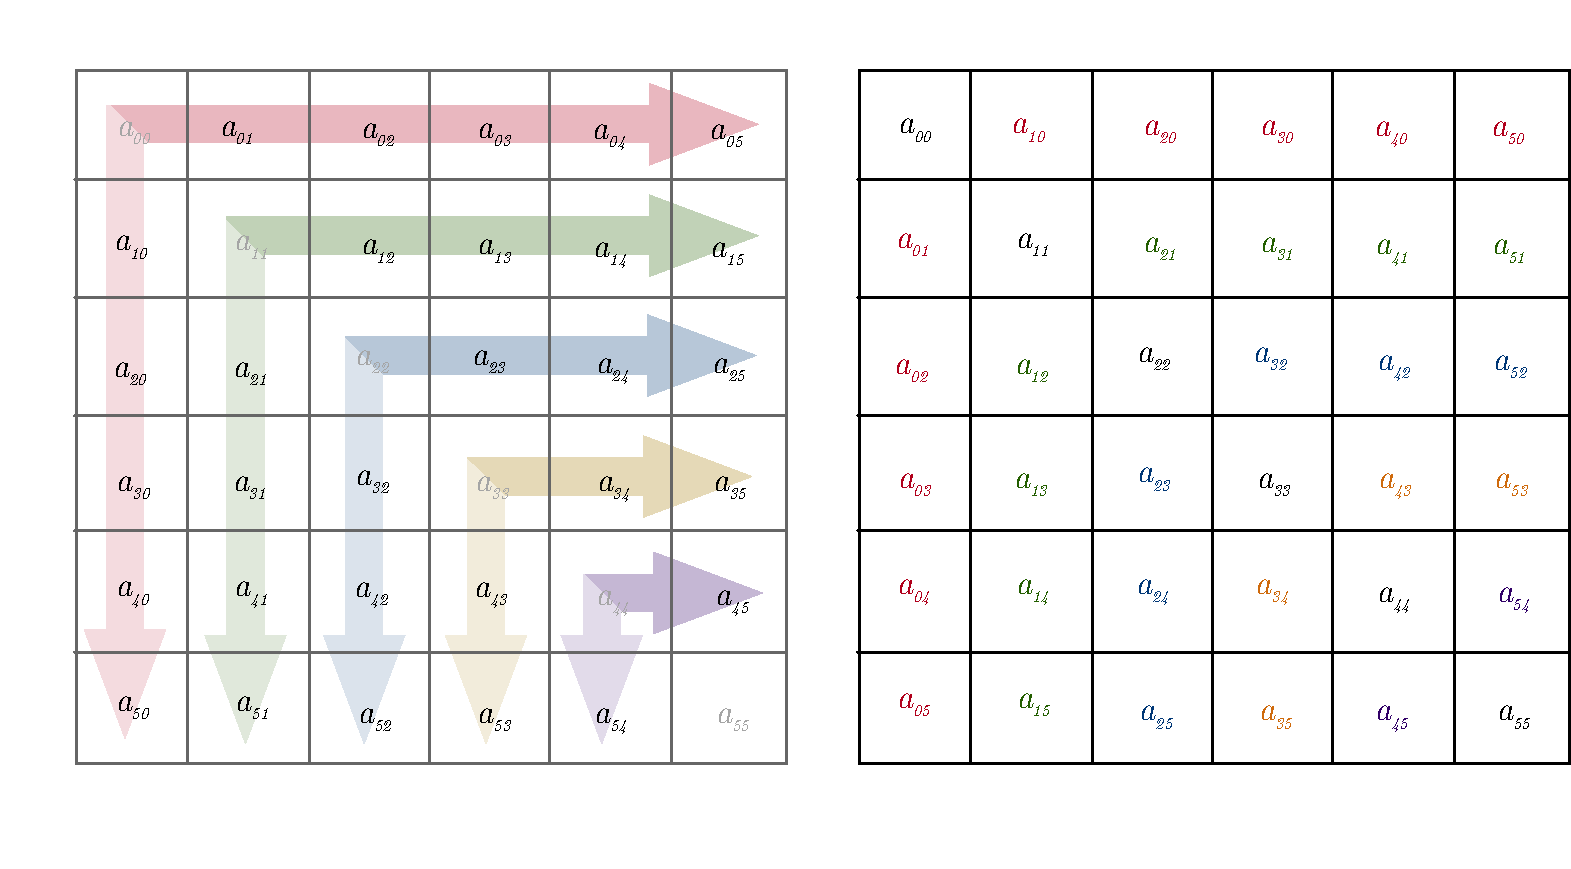
\includegraphics[width=1\linewidth]{images/diagonal-threaded.pdf}}
    \vspace{-20pt}
    \caption{Threaded diagonal matrix transposition}
    \label{fig:diagonal_transpose}
\end{Figure}%
\vspace{10pt}

\vspace{5pt}
\begin{algorithm}[H]
    \small
    \caption{Diagonal OpenMP Algorithm}\label{pc:omp-diag}
    	\SetAlgoLined
     	\KwIn{Matrix A (N x N)}
    	\KwOut{$A^T$}
	$N \leftarrow$ size of A \\
	Parallelize \textbf{for} loop using OpenMP \\
	\For{i = 0 to (N-1)}{
		\For{j = i+1 to (N-1)}{
			\If{i != j}{Swap $A_{i,j}$ and $A_{j,i}$}\
		}
	}
	\vspace{6pt}
\end{algorithm}%
\vspace{5pt}

This method performs significantly worse than a serial method for a small matrix of size 64x64, but has much faster execution speed than serial code for all other larger matrices that were tested.

%--------------------------------------------------------------------------------------
\subsection{Block-Oriented Swap}
In a block-oriented transpose, the square matrix is subdivided into blocks consisting of 2x2 sub-matrices. The matrix elements corresponding to each  block are then ``transposed'' (their placement is swapped by reversing their row/column) as shown in Figure \ref{fig:block-transpose}. The elements inside these transposed sub-matrices are then transposed with three operations per block. If the block lies along the diagonal, then the first swap is not performed, and the elements inside the block are transposed with a constant three operation per block. This results in a final transposed matrix.  

\begin{Figure}
    \centering
    \vspace{10pt}
    {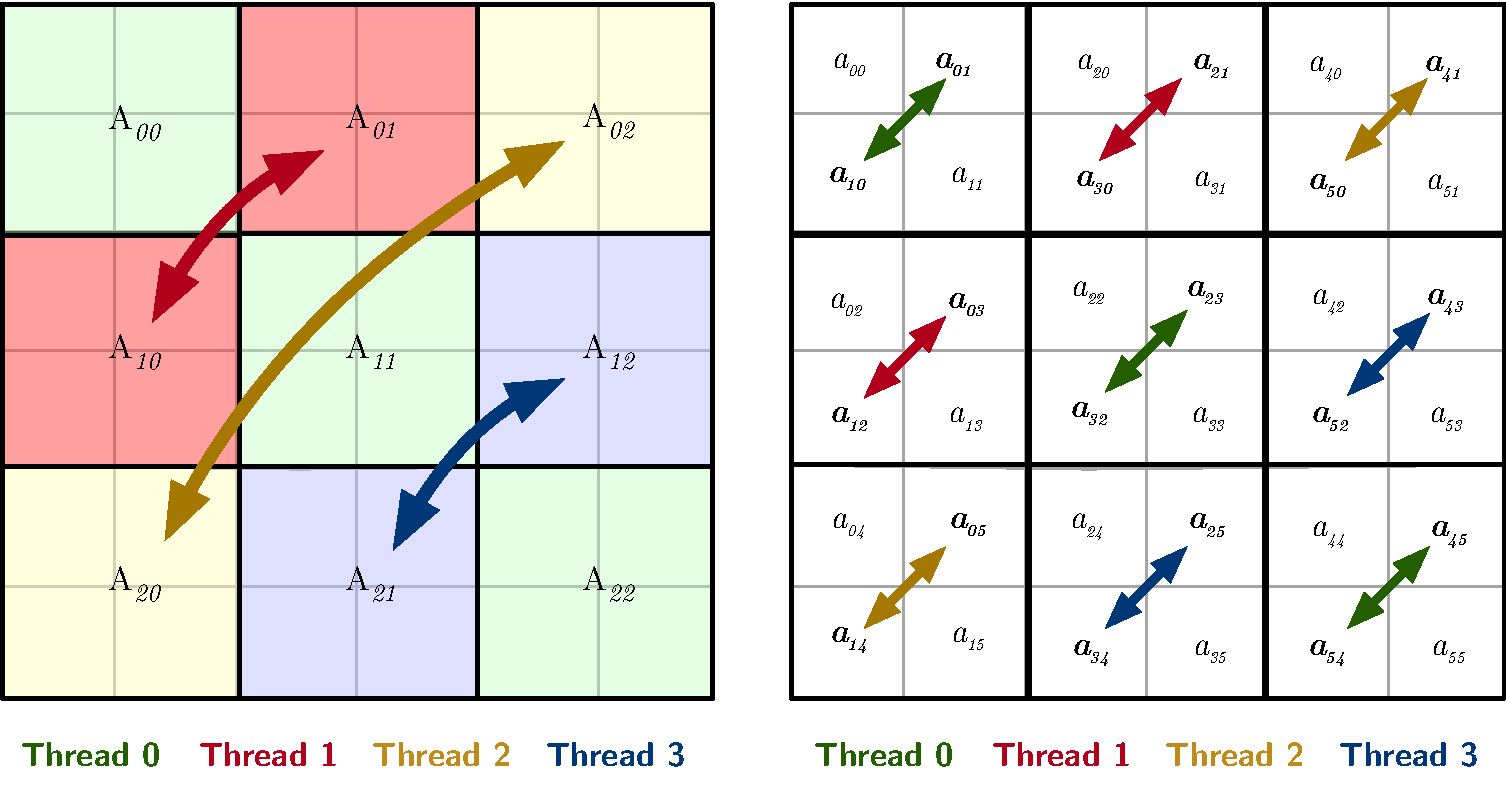
\includegraphics[width=1\linewidth]{images/block-oriented.pdf}}
    \caption{Threaded block-oriented matrix transposition}
    \label{fig:block-transpose} 
    \vspace{15pt}
\end{Figure}%

Algorithm \ref{pc:omp-block} describes this transposition method in pseudocode, which is implemented as shown in Appendix II, Code Listing \ref{code:transpose}. In the implementation, the mapping between element positions within a sub-matrix block is explicitly mapped by indices, and performed with the use of a temporary variable, using $\mathcal{O}(1)$ storage per thread.

\vspace{5pt}
\begin{algorithm}[H]
    \small
    \caption{Block OpenMP Algorithm}\label{pc:omp-block}
    	\SetAlgoLined
     	\KwIn{Matrix A (N x N)}
    	\KwOut{$A^T$}
	$N \leftarrow$ size of A
	Declare variable \texttt{stride} $\leftarrow 2$
	Parallelize \textbf{for} loop using OpenMP
	\For{\texttt{row} = 0 to (N-1), increment by \texttt{stride}}{
		\For{\texttt{col} = 0 to \texttt{row}, increment by \texttt{stride}}{
			\uIf{\texttt{row} == \texttt{col}}{
			    $\texttt{temp} \leftarrow A_{row+1, col+1}$ \\
			    $A_{row+1, col} \leftarrow A_{row, col+1}$ \\
			    $A_{row, col+1} \leftarrow  \texttt{temp}$ \\
			    }
			\Else{
			    \For{i = 0 to \texttt{stride}-1}{
			        \For{j = 0 to \texttt{stride}-1}{
			            $\texttt{temp} \leftarrow A_{col+j, row+i}$\\
			            $A_{col+j, row+i} \leftarrow A_{row+i, col+j}$\\
			            $A_{row+i, col+j} \leftarrow  \texttt{temp}$\\
			        }
			    }
			}
		}
	}
	\vspace{3pt}
\end{algorithm}%
\vspace{5pt}

By exploiting greater data locality, the parallel method increases performance, but performs well even with with small matrices.

%%%%%%%%%%%%%%%%%%%%%%%%%%%%%%%%%%%%%%%%%%%%%%%%%%%%%%%%%%%%%%%%%%%%%%%%%%%%%%%%%%%%%%%
\section{PThread}
Threads are an assembly of instructions which are arranged to execute in a via an operating system \cite{lewis1996pthreads}.The relationship of multiple threads to a single process are analogous to multiple processes in a single shell. PThreads are classified as a group of C-programming types and processes which can be implemented from the specification, in this report using the \verb|pthread.h| header file \cite{lewis1996pthreads}. Unlike OpenMP, which creates, joins and destroys threads with simple pragma directives, the pthreads library requires lower level control, requiring manual setup, allocation, synchronisation and destruction of threads through the Pthreads public interface of function calls. The resulting MT code is often more complicated and not as easy to read as an OpenMP MT implementation.

%--------------------------------------------------------------------------------------
\subsection{Thread functions}
The mechanism of calling a function for a thread to execute requires passing the function at time o thread creation, and any arguments to the function must also be passed as type (\verb|void *|). In the case of multiple arguments, this imposes the requirement to pass the arguments inside a \verb|struct|, increasing the complexity of the codebase, and therefore the difficulty of reading, understanding and maintaining the code. The implementation is shown in Appendix II, Code Listing \ref{code:transpose}. Each thread has its own stack and associated counters, but have shared access to all open memory and files. As thread execution time can not be determined exactly, care must be taken to prevent errors by manually locking access to critical sections of code execution when necessary. This would require enforcing a serial execution restriction within a critical access section. 

%--------------------------------------------------------------------------------------
\subsection{Na\"ive Implementation}
The ``na\"ive'' transposition algorithm uses the same nested \textit{for} loop structure from the basic serial implementation, but instead of a single thread performing all swaps sequentially, the row traversal is split into equally sized sections for each thread. This operation is illustrated in Figure \ref{fig:thread_creation}. Although the resulting sections have a block-like structure in their traversal, there is little no advantage taken by processor cache, and it is very similar to the diagonally-oriented transposition method and has similar performance, as seen in the timing shown in Appendix I, Table \ref{tab:timing}. The method is included in the timing and code implementation for completeness, and offers no significant advantages over the similarly performing diagonal method discussed below. The individual thread action is a function with signature \verb|void *naiveThreadAction(void *args)|, which is passed a pointer to a struct of type \verb|matrix_args|, which contains a pointer to the main Matrix array, and two integer values used as the start and end row indices for each thread section.

\vspace{12pt}
\begin{Figure}
    % \hspace{-10pt}
    {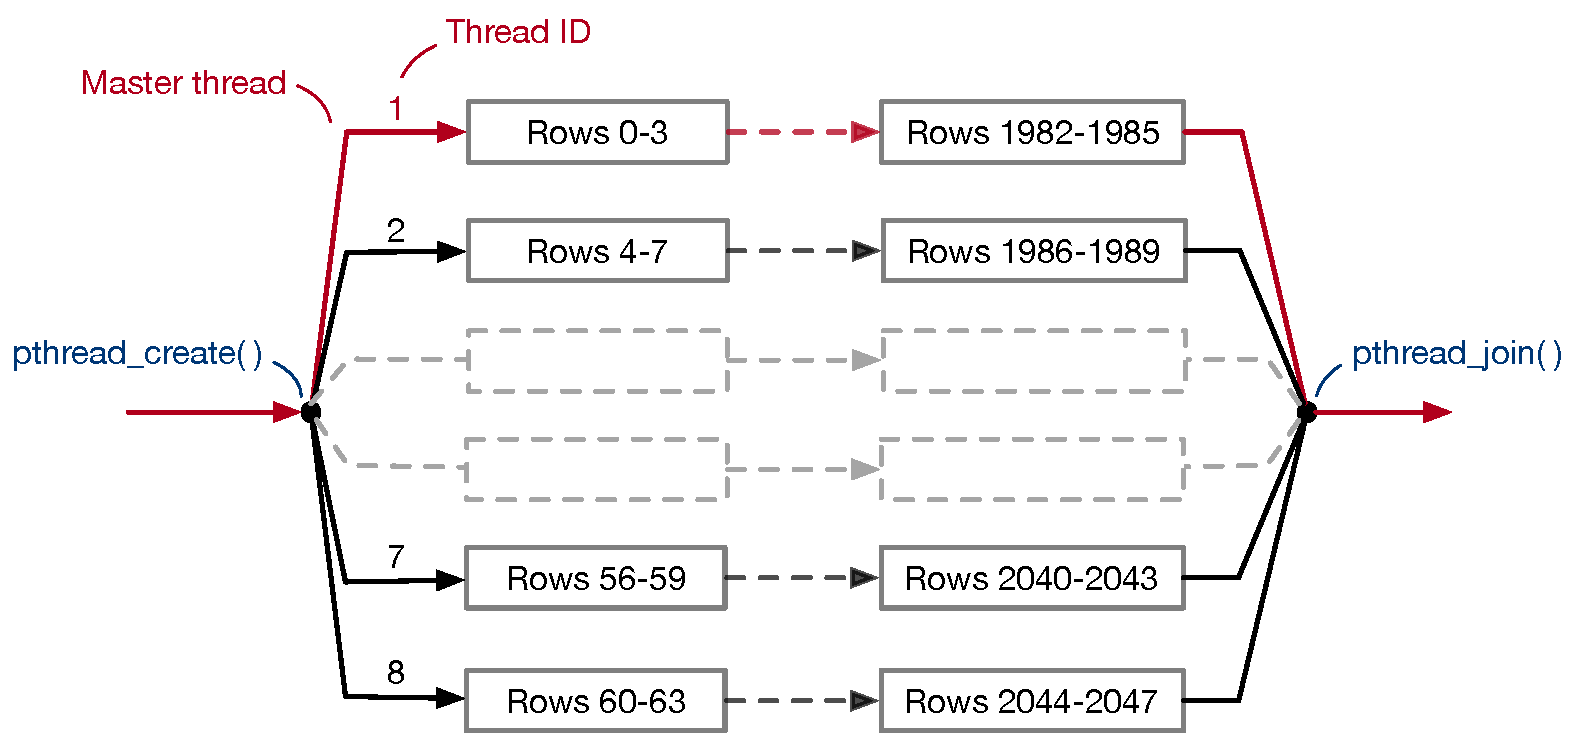
\includegraphics[width=1\linewidth]{images/threads.pdf}}
    % \vspace{5pt}
    \caption{PThread creating and joining}
    \label{fig:thread_creation}
\end{Figure}%
% \vspace{5pt}

%--------------------------------------------------------------------------------------
\subsection{Diagonal Swap}
The PThreaded algorithm is applied to transpose a matrix by swapping rows and columns along the main diagonal of the input matrix. The main transpose function, \verb|transposeMatrixDiagonalPThread()| sets up a number of threads (for fair timing the number of threads is taken from the same environment variable \verb|OMP_NUM_THREADS| used by OpenMP) and then each thread calls \verb|diagonalThreadAction()| to proceed along along a certain section of the diagonal of the matrix. Each thread takes a single row and column, and sequentially swaps each element to perform the transpose. If the number of threads is not a integer multiple of $N$, then there will be idle threads near the end of the diagonal traversal. When all threads have completed their tasks (none of which simultaneously access the same data elements in the matrix), then the threads are joined in another \textit{for} loop, and the memory allocated to the threads are released.
The method suffers from the same poor performance with small arrays, but performs well with larger input matrices. It has near-identical performance to the diagonal OpenMP algorithm.

%--------------------------------------------------------------------------------------
\subsection{Block-Oriented Swap}
Similarly to the OpenMP operation discussed in \cref{sec:diagonal_omp}, the pthreads algorithm \verb|transposeMatrixBlockPThread()| transposes a matrix by swapping blocks of sub-matrices above and below the main diagonal blocks, followed by a further element-wise transposition of all non-diagonal elements in all sub-matrices (including the main diagonal sub-matrices). The implemented function splits up the main matrix into blocks of 2x2, and assigns a threads to each block up to the maximum number of threads. When each thread completes its task, it picks up another un-swapped/un-transposed sub-matrix block. Once all threads have completed their jobs (and all elements in the matrix have been moved into their new transposed indices, then the threads are joined and the allocated memory is released.

The method performs poorly on small arrays but with arrays where $N>2048$, the parallel algorithm performs as well as the OpenMP block-oriented algorithm.
%%%%%%%%%%%%%%%%%%%%%%%%%%%%%%%%%%%%%%%%%%%%%%%%%%%%%%%%%%%%%%%%%%%%%%%%%%%%%%%%%%%%%%%
\section{Timing and results}
The measured CPU times for the implemented algorithms, run over arrays between $N=2^5$ and $N=2^15$ are are summarised in Appendix I, Table \ref{tab:timing}. Timing was performed using \verb|steady_clock| provided by the \verb|chrono| library. This clock is monotonic, and is designed to measure differences in physical time, not CPU operations, and is immune to sleep or idle operations. These properties make it suitable to measure threaded and non-threaded performance of algorithms. The timings were run with \verb|OMP_NUM_THREADS=8| on a four-core i7 Macbook Pro running OSX 10.14.3 with 16 Gb of 1600 MHz RAM.

%--------------------------------------------------------------------------------------
\subsection{Discussion of Results}
As noted in the tabulated results shown in Table \ref{tab:timing}, the block-oriented algorithms completed their instructions with faster timings than the serial and na\"ive implementations. The times recorded show that the diagonal implementation using PThreads (very) slightly outperforms OpenMP. However OpenMP outperforms PThreads when using the block-oriented algorithm for smaller arrays, but this result depends on the matrix size used. As the array size increases, PThreads performs slightly better. The results are inconclusive regarding the optimal strategy for parallel transposition of power-of-two square matrices with $N>4096$. One explanation of the ambiguity of the measured results could be that the implemented code does not take the concept of "false sharing" into consideration. When one thread affects the performance of another thread it is referred to as false sharing [\cite{FalseSharing:URL}]. As the number of threads rises, so too does the number of false sharing cases. To resolve this concern, inclusion of padding in the code should be addressed which in turn guarantees that threads will gain access to separate cache lines. 
\vspace{20pt} %

%%%%%%%%%%%%%%%%%%%%%%%%%%%%%%%%%%%%%%%%%%%%%%%%%%%%%%%%%%%%%%%%%%%%%%%%%%%%%%%%%%%%%%%
\section{Conclusion}
This laboratory exercise focuses on the notion of parallel programming through the utilisation of OpenMP and PThreads. OpenMP has been explored by performing matrix transposition using a naive implementation, diagonally-directed swapping, and a block-oriented swap and transpose algorithm. PThreads has been explored using the same algorithms, but with manual creation and joining of the same number of threads. 

%--------------------------------------------------------------------------------------
\balance
\end{multicols}
% \clearpage
% \newpage
% \onecolumn

\vfill

% -------------------------------------------------------------------------------------
% 	BIBLIOGRAPHY
% ------------------------------------------------------------------------------------
\bibliographystyle{IEEEtran}
{\bibliography{IEEEabrv,ELEN4020_Lab_2_Report.bib}}

%-------------------------------------------------------------------------------------
%	APPENDICES
%-------------------------------------------------------------------------------------
\newgeometry{left=1.2cm,right=1.2cm,top=1cm,bottom=1.3cm}
\onecolumn
\renewcommand{\thefigure}{A\arabic{figure}}
\renewcommand{\thetable}{A\arabic{table}}
\renewcommand{\thelstlisting}{A\arabic{lstlisting}}
% \renewcommand\thesection{\c{section}}
% \renewcommand{\thesubsection}{\Alph{subsection}}

\setcounter{figure}{0}
\begin{appendices}
\section{} \label{app:I}
% \rule{0.975\textwidth}{.4pt}

\vspace{20pt}

\begin{table}[ht] \centering
    \renewcommand\tabcolsep{8pt} %
    \def\arraystretch{1.35}%
    \caption{Measured algorithm execution CPU time [$\mu s$]}
    \label{tab:timing}
    \small{%
    \hspace{-10pt}
    \vspace{5pt} \hfill
    \begin{tabular}{@{}crrrrrrr@{}} \toprule
        \multicolumn{1}{@{}c}{\multirow{3}{*}{$\mathbf{N_{o} = N_{1}}$}} & %
        \multicolumn{1}{@{}c}{\multirow{3}{*}{\textbf{Serial}}} & %
        \multicolumn{3}{@{}c}{\textbf{PThread}} & %
        \multicolumn{3}{@{}c}{\textbf{OpenMP}}  \\ 
        %
        & & \multicolumn{3}{@{}c}{$\overbrace{\hspace{160pt}}$} & %
        \multicolumn{3}{@{}c}{$\overbrace{\hspace{160pt}}$} \\
        & & \multicolumn{1}{@{}c}{Na\"ive} & %
        \multicolumn{1}{@{}c}{Diagonal} & %
        \multicolumn{1}{@{}c}{Block} & %
        \multicolumn{1}{@{}c}{Na\"ive} & %
        \multicolumn{1}{@{}c}{Diagonal} & %
        \multicolumn{1}{@{}c}{Block} \\ \midrule
        %  128	&	471		&	298		&	375		&	272		&	287		&	327		\\
        % 1024	&	24041	&	7112	&	7234	&	7292	&	6688	&	5882	\\
        % 2048	&	132453	&	30707	&	35785	&	29095	&	35093	&	25846	\\
        % 4096	&	685683	&	158552	&	156639	&	128497	&	171226	&	124326	\\ \bottomrule
        %
        % micro seconds below
	64 & $5.8000\times 10^1$ & $8.8900\times 10^2$ & $1.1000\times 10^2$ & $8.8000\times 10^1$ & $2.6700\times 10^2$ & $1.8900\times 10^2$ & $2.0800\times 10^2 $\\
    128 & $2.3800\times 10^2$ & $1.9400\times 10^2$ & $2.6400\times 10^2$ & $1.7000\times 10^2$ & $2.4900\times 10^2$ & $2.2400\times 10^2$ & $2.7100\times 10^2$ \\
    256 & $9.5200\times 10^2$ & $7.0500\times 10^2$ & $6.2100\times 10^2$ & $4.8800\times 10^2$ & $8.4400\times 10^2$ & $6.6600\times 10^2$ & $7.2700\times 10^2$ \\
    512 & $4.8150\times 10^3$ & $2.3750\times 10^3$ & $2.3780\times 10^3$ & $1.6690\times 10^3$ & $1.8000\times 10^3$ & $2.3150\times 10^3$ & $2.7880\times 10^3$ \\
    1024 & $2.4807\times 10^4$ & $8.7550\times 10^3$ & $7.4380\times 10^3$ & $5.9310\times 10^3$ & $6.3070\times 10^3$ & $9.5170\times 10^3$ & $7.5420\times 10^3$ \\
    2048 & $1.3589\times 10^5$ & $3.5944\times 10^4$ & $3.8697\times 10^4$ & $3.0029\times 10^4$ & $4.0392\times 10^4$ & $3.3908\times 10^4$ & $2.4795\times 10^4$ \\
    4096 & $7.1511\times 10^5$ & $1.7276\times 10^5$ & $1.6319\times 10^5$ & $1.3432\times 10^5$ & $1.6092\times 10^5$ & $1.6682\times 10^5$ & $1.3212\times 10^5$ \\
    8192 & $3.0509\times 10^6$ & $7.6561\times 10^5$ & $7.5487\times 10^5$ & $6.5091\times 10^5$ & $7.6296\times 10^5$ & $7.5997\times 10^5$ & $5.5517\times 10^5$ \\
    16384 & $1.2585\times 10^7$ & $3.3533\times 10^6$ & $3.2589\times 10^6$ & $2.6138\times 10^6$ & $3.2283\times 10^6$ & $3.2886\times 10^6$ & $2.2703\times 10^6$ \\
    32768 & $9.0450\times 10^7$ & $1.8300\times 10^7$ & $1.8769\times 10^7$ & $1.2127\times 10^7$ & $1.7252\times 10^7$ & $1.7936\times 10^7$ & $1.1369\times 10^7$ \\ \bottomrule
% %
% % milli seconds below
%   64	& $5.8000\times 10^{-2}$ & $8.8900\times 10^{-1}$ & $1.1000\times 10^{-1}$ & $8.8000\times 10^{-2}$ & $2.6700\times 10^{-1}$ & $1.8900\times 10^-{01}$ & $2.0800\times 10^{-1}$ \\
%   128	& $2.3800\times 10^{-1}$ & $1.9400\times 10^{-1}$ & $2.6400\times 10^{-1}$ & $1.7000\times 10^{-1}$ & $2.4900\times 10^{-1}$ & $2.2400\times 10^-{01}$ & $2.7100\times 10^{-1}$ \\
%   256	& $9.5200\times 10^{-1}$ & $7.0500\times 10^{-1}$ & $6.2100\times 10^{-1}$ & $4.8800\times 10^{-1}$ & $8.4400\times 10^{-1}$ & $6.6600\times 10^-{01}$ & $7.2700\times 10^{-1}$ \\
%   512	& $4.8150\times 10^{0}$  & $2.3750\times 10^{0}$  & $2.3780\times 10^{0}$  & $1.6690\times 10^{0}$  & $1.8000\times 10^{0}$  & $2.3150\times 10^{0}$   & $2.7880\times 10^{0}$ \\
%   1024 	& $2.4807\times 10^{1}$  & $8.7550\times 10^{0}$  & $7.4380\times 10^{0}$  & $5.9310\times 10^{0}$  & $6.3070\times 10^{0}$  & $9.5170\times 10^{0}$   & $7.5420\times 10^{0}$ \\
%   2048 	& $1.3589\times 10^{2}$  & $3.5944\times 10^{1}$  & $3.8697\times 10^{1}$  & $3.0029\times 10^{1}$  & $4.0392\times 10^{1}$  & $3.3908\times 10^{1}$   & $2.4795\times 10^{1}$ \\
%   4096 	& $7.1511\times 10^{2}$  & $1.7275\times 10^{2}$  & $1.6319\times 10^{2}$  & $1.3432\times 10^{2}$  & $1.6092\times 10^{2}$  & $1.6682\times 10^{2}$   & $1.3212\times 10^{2}$ \\
%   8192 	& $3.0509\times 10^{3}$  & $7.6561\times 10^{2}$  & $7.5487\times 10^{2}$  & $6.5091\times 10^{2}$  & $7.6296\times 10^{2}$  & $7.5997\times 10^{2}$   & $5.5517\times 10^{2}$ \\
%   16384 & $1.2585\times 10^{4}$  & $3.3533\times 10^{3}$  & $3.2589\times 10^{3}$  & $2.6138\times 10^{3}$  & $3.2283\times 10^{3}$  & $3.2886\times 10^{3}$   & $2.2703\times 10^{3}$ \\
%   32768 & $9.0450\times 10^{4}$  & $1.8300\times 10^{4}$  & $1.8769\times 10^{4}$  & $1.2127\times 10^{4}$  & $1.7252\times 10^{4}$  & $1.7936\times 10^{4}$   & $1.1369\times 10^{4}$ \\ \bottomrule
    \end{tabular} \hfill}
\end{table}

\vspace{50pt}

\begin{figure}[h] \centering
    {\hspace{-30pt}%
    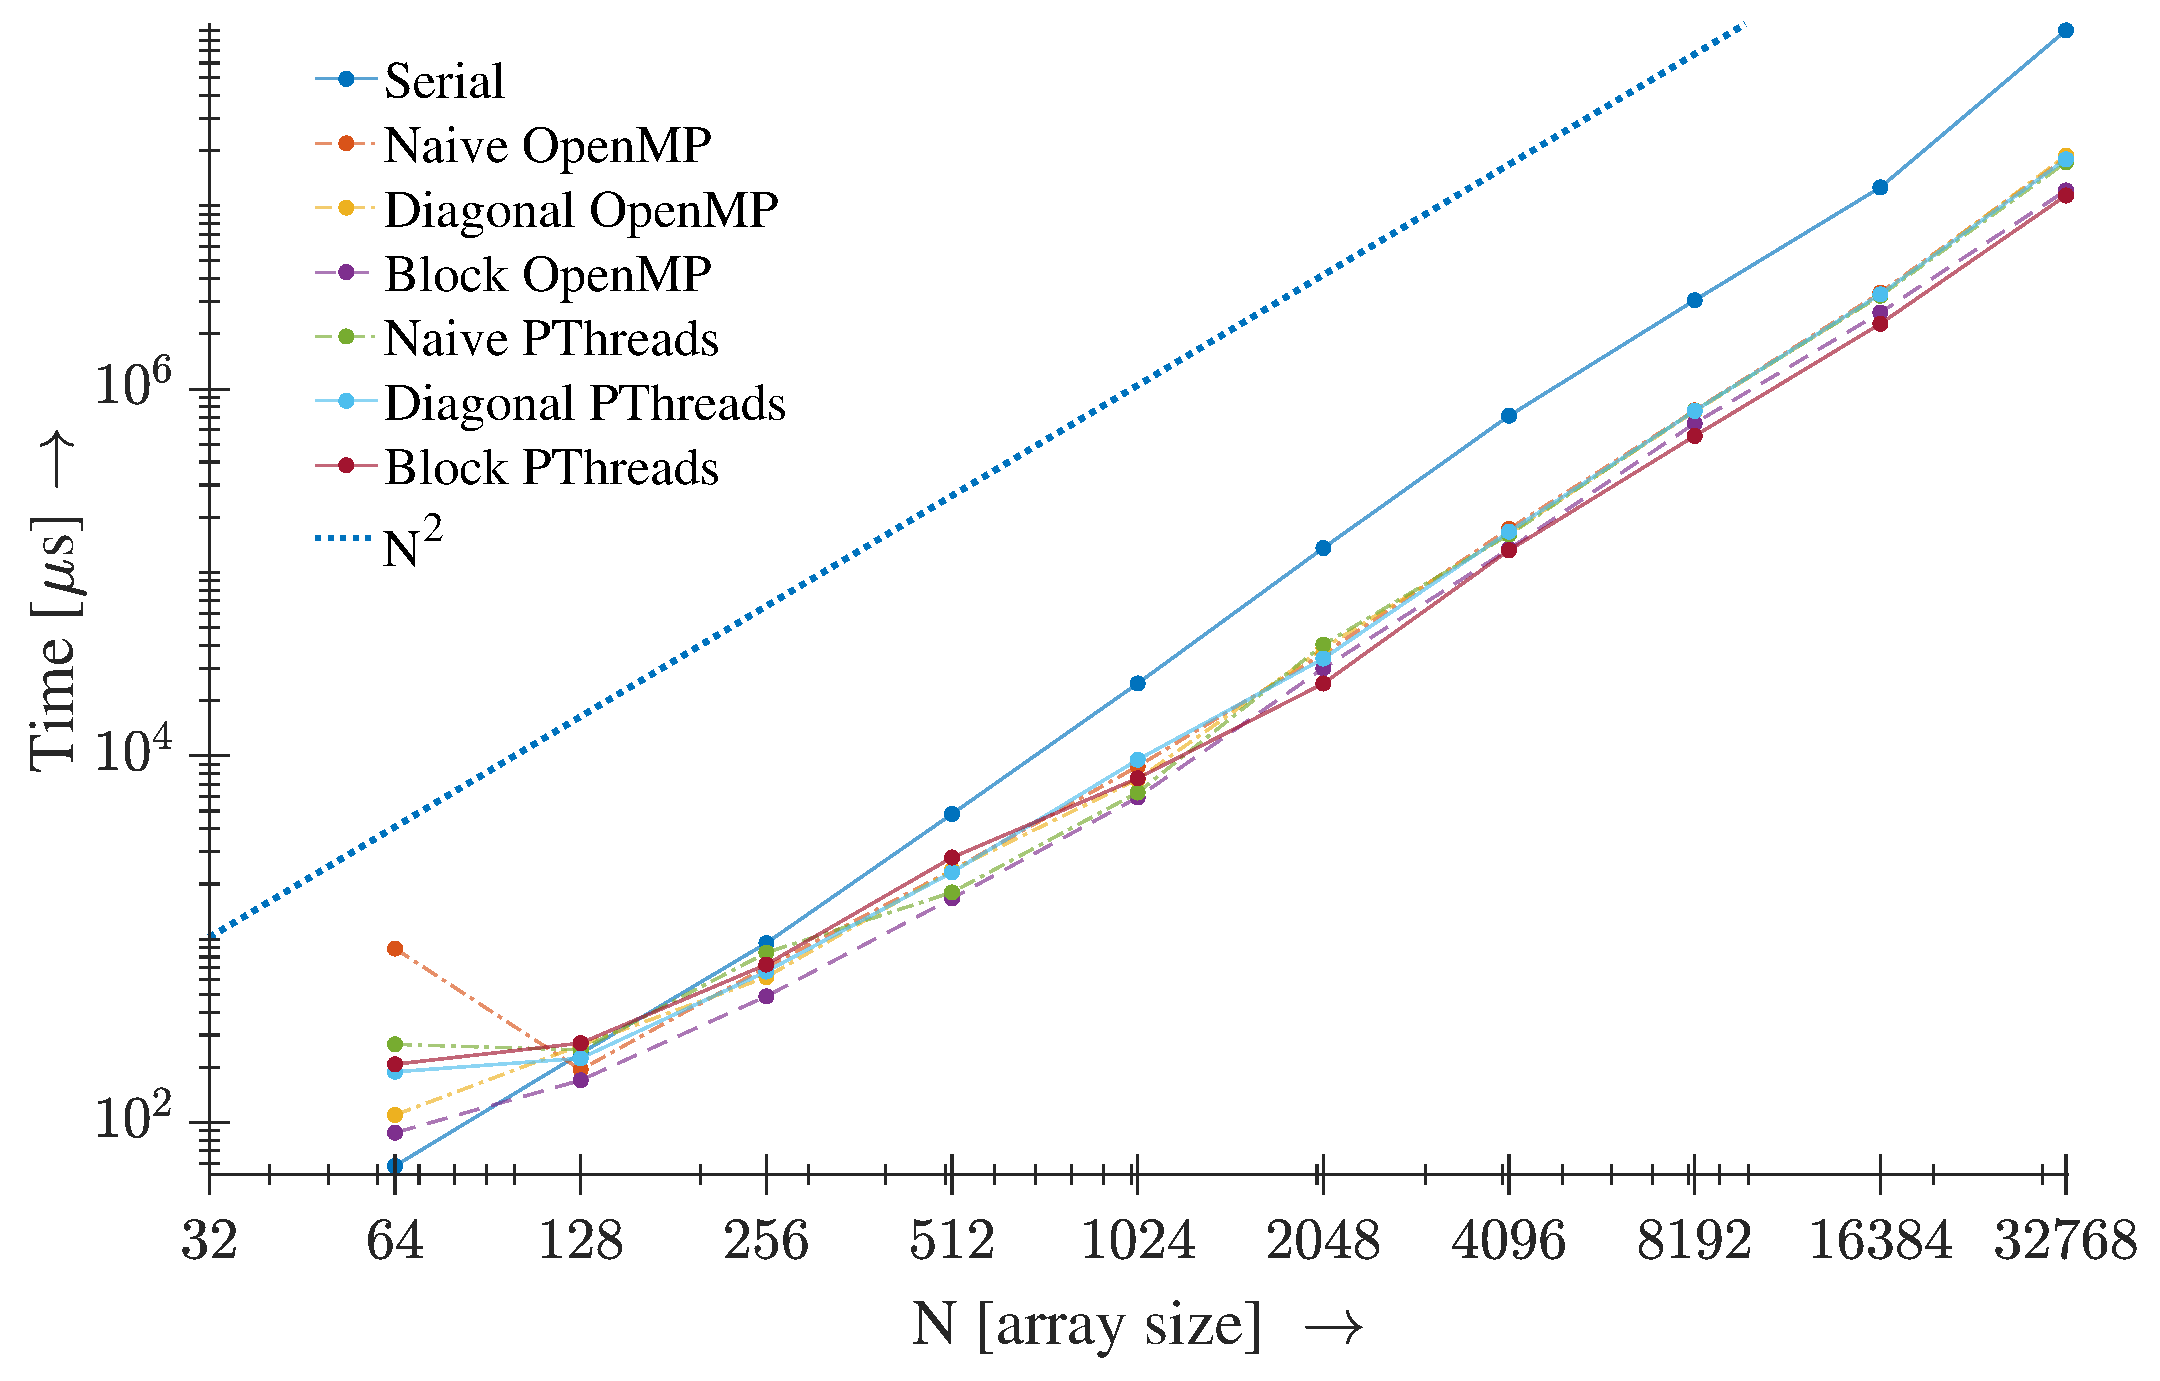
\includegraphics[width=0.95\linewidth]{images/asymptotic.eps}}
    \caption{Computational time vs array size (log plot)}
    \label{fig:big_o} 
    % \vspace{-10pt}
\end{figure}

\newpage
\section{} \label{app:II}

{{\fontfamily{fi4}\selectfont ...} % Use Inconsulata font
\captionof{lstlisting}{Matrix.h}
\rule{0.975\textwidth}{.6pt}
\lstinputlisting[language=C++]{code/Matrix.h}\label{code:matrix}

\newpage

\captionof{lstlisting}{lab2.cpp}
\rule{0.975\textwidth}{.6pt}
\lstinputlisting[language=C++]{code/lab2.cpp}\label{code:lab2}
\rule{0.975\textwidth}{.4pt}

\vspace{15pt}

\captionof{lstlisting}{transpose.cpp}
\rule{0.975\textwidth}{.6pt}
\lstinputlisting[language=C++]{code/transpose.cpp}\label{code:transpose}

\newpage
\vspace{-50pt}
\captionof{lstlisting}{utilities.cpp}
\rule{0.975\textwidth}{.6pt}
\lstinputlisting[language=C++]{code/utilities.cpp}\label{code:utility}
}

\end{appendices}

\end{document}